\documentclass[tikz,border=2pt]{standalone}
% Preámbulo común de los diagramas TikZ (misma paleta y letra que las notas)
\usepackage[T1]{fontenc}\usepackage[utf8]{inputenc}
\usepackage{libertinus}\usepackage{libertinust1math}
\usepackage[defaultsans,scale=0.92]{lato}
\usepackage{amsmath,amssymb,bm}
\usepackage{tikz}\usetikzlibrary{calc,positioning,arrows.meta,shapes.geometric,decorations.pathreplacing,decorations.pathmorphing,fit,backgrounds}
\definecolor{snlazul}{HTML}{1E5AA8}\definecolor{snlnoche}{HTML}{14213D}\definecolor{snlvioleta}{HTML}{6C4AB6}
\definecolor{snlcoral}{HTML}{D1495B}\definecolor{snlambar}{HTML}{E09F3E}\definecolor{snlverde}{HTML}{2A9D8F}
\definecolor{snlteal}{HTML}{0F7173}\definecolor{snlgris}{HTML}{5C677D}\definecolor{snlfondo}{HTML}{F4F6FA}
\tikzset{>={Stealth[length=2.2mm]},
  bloque/.style={draw=#1,fill=#1!8,thick,rounded corners=2pt,minimum height=11mm,minimum width=20mm,align=center,font=\small},
  bloque/.default=snlazul,
  suma/.style={draw=snlnoche,thick,circle,inner sep=0pt,minimum size=5mm},
  flecha/.style={->,thick,draw=snlnoche},
  etq/.style={font=\small,text=snlnoche},
  nota/.style={font=\footnotesize\sffamily,text=snlgris,align=center}}

\begin{document}
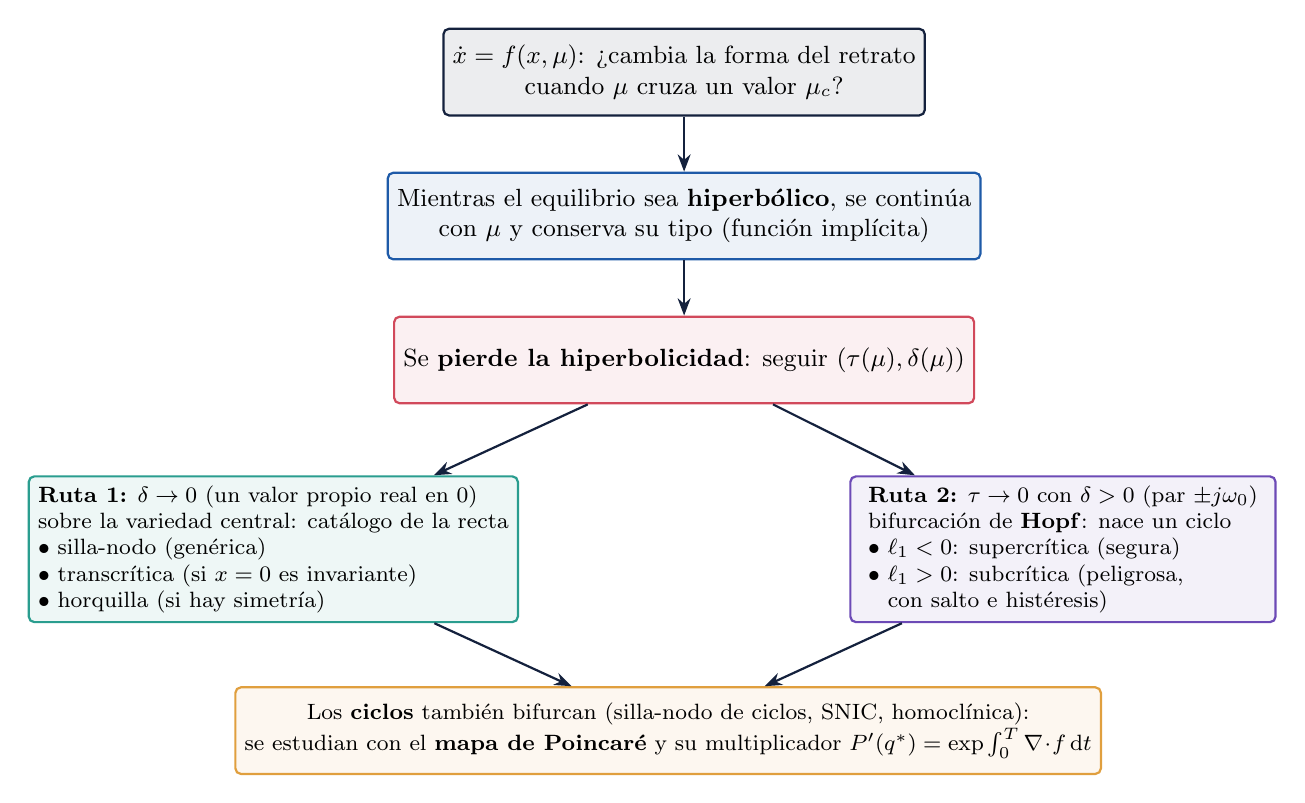
\begin{tikzpicture}[node distance=6mm and 8mm]
 \node[bloque=snlnoche,minimum width=60mm] (q) {$\dot x=f(x,\mu)$: ¿cambia la forma del retrato\\ cuando $\mu$ cruza un valor $\mu_c$?};
 \node[bloque=snlazul,below=7mm of q,minimum width=60mm] (hip) {Mientras el equilibrio sea \textbf{hiperbólico}, se continúa\\ con $\mu$ y conserva su tipo (función implícita)};
 \node[bloque=snlcoral,below=7mm of hip,minimum width=60mm] (pierde) {Se \textbf{pierde la hiperbolicidad}: seguir $(\tau(\mu),\delta(\mu))$};
 \node[bloque=snlverde,below left=9mm and -16mm of pierde,minimum width=54mm,align=left,font=\footnotesize] (r1) {\textbf{Ruta 1:} $\delta\to0$ (un valor propio real en $0$)\\ sobre la variedad central: catálogo de la recta\\ $\bullet$ silla-nodo (genérica)\\ $\bullet$ transcrítica (si $x=0$ es invariante)\\ $\bullet$ horquilla (si hay simetría)};
 \node[bloque=snlvioleta,below right=9mm and -16mm of pierde,minimum width=54mm,align=left,font=\footnotesize] (r2) {\textbf{Ruta 2:} $\tau\to0$ con $\delta>0$ (par $\pm j\omega_0$)\\ bifurcación de \textbf{Hopf}: nace un ciclo\\ $\bullet$ $\ell_1<0$: supercrítica (segura)\\ $\bullet$ $\ell_1>0$: subcrítica (peligrosa,\\ \phantom{$\bullet$} con salto e histéresis)};
 \node[bloque=snlambar,below=8mm of $(r1.south)!0.5!(r2.south)$,minimum width=100mm,font=\footnotesize] (cic) {Los \textbf{ciclos} también bifurcan (silla-nodo de ciclos, SNIC, homoclínica):\\ se estudian con el \textbf{mapa de Poincaré} y su multiplicador $P'(q^*)=\exp\int_0^T\nabla\!\cdot\! f\,\mathrm dt$};
 \draw[flecha] (q) -- (hip); \draw[flecha] (hip) -- (pierde);
 \draw[flecha] (pierde) -- (r1); \draw[flecha] (pierde) -- (r2);
 \draw[flecha] (r1) -- (cic); \draw[flecha] (r2) -- (cic);
\end{tikzpicture}
\end{document}
